% !TEX encoding = UTF-8 Unicode
\documentclass[review]{elsarticle}

% table properties
\usepackage{booktabs}
\usepackage{caption}
\usepackage{subcaption}
\usepackage{color, colortbl}
\definecolor{LightCyan}{rgb}{0.88,1,1}
% table position
\usepackage{float}
\restylefloat{table}

\usepackage{lineno,hyperref}
\modulolinenumbers[5]

\journal{Journal of \LaTeX\ Templates}

%%%%%%%%%%%%%%%%%%%%%%%
%% Elsevier bibliography styles
%%%%%%%%%%%%%%%%%%%%%%%
%% To change the style, put a % in front of the second line of the current style and
%% remove the % from the second line of the style you would like to use.
%%%%%%%%%%%%%%%%%%%%%%%

%% Numbered
%\bibliographystyle{model1-num-names}

%% Numbered without titles
%\bibliographystyle{model1a-num-names}

%% Harvard
%\bibliographystyle{model2-names.bst}\biboptions{authoryear}

%% Vancouver numbered
%\usepackage{numcompress}\bibliographystyle{model3-num-names}

%% Vancouver name/year
\usepackage{numcompress}\bibliographystyle{model4-names}\biboptions{authoryear}

%% APA style
%\bibliographystyle{model5-names}\biboptions{authoryear}

%% AMA style
%\usepackage{numcompress}\bibliographystyle{model6-num-names}


%% `Elsevier LaTeX' style
%\bibliographystyle{elsarticle-num}
%\u{g} – g
%\u{G} – g
%\c{c} – ç
%\c{C} – Ç
%\c{s} – ş
%\c{S} – Ş
%\"{u} – ü
%\"{U} – Ü
%\"{o} – ö
%\"{O} – Ö
%{\i} – ı
%\.{I} – İ
%\^{a}
%\^{A}

%%%%%%%%%%%%%%%%%%%%%%%

\begin{document}

\begin{frontmatter}

\title{A New Approach for Detection of Moving Objects in FITS Images: A-Track}

%% Group authors per affiliation:

\author[ubt]{T.~Atay}
\ead{tolgaphd@gmail.com}
\author[ubt]{M.~Kaplan}
\author[ubt]{Y.~K{\i}l{\i}\c{c}}
\author[ubt]{N.~Karap{\i}nar}

\address[ubt]{Akdeniz Universitesi, Fen Fakultesi, Uzay Bilimleri ve Teknolojileri Bolumu, Antalya, Turkiye}

\begin{abstract}
We have developed an open-source, cross-platform pipeline for the detection of moving objects such as asteroids or comets in sequential telescope images. We tested the pipeline using the T\"{U}B\.{I}TAK National Observatory data which were acquired by a 1.0 meter diameter telescope (T100) and an SI CCD 1100 camera. We found that our pipeline is at least as successful as any other software used for asteroid detection, in terms of detection efficiency, stability, and processing time.

{\bf Program summary}

{\em Program title: A-TRACK

Catalogue identifier: a-track\_v1\_0

Program summary URL: https://github.com/akdeniz-uzay/A-Track

Program obtainable from: https://github.com/akdeniz-uzay/A-Track/archive/master.zip

Licensing provisions: Standard GNU General Public Licence, http://www.gnu.org/licenses/gpl-3.0.en.html

No. of lines in distributed program, including test data, etc.: 

No. of bytes in distributed program, including test data, etc.: 

Distribution format: .zip

Programming language: Python.

Computer: Personal Computer.

Operating system: Any OS where Python \ldots\ldots are installed.

RAM: Around \ldots Mbytes

Classification: \ldots

External routines: numpy \ldots

Subprograms used: 

Nature of problem: 

Solution method:

Restrictions:

Running time:
}
\end{abstract}

\begin{keyword}
  methods: data analysis \sep minor planets \sep asteroids \sep techniques: image processing
  \MSC[2015] 10-13\sep  99-00
\end{keyword}

\end{frontmatter}

%\linenumbers

\section{Introduction}

Asteroids and comets offer valuable information about the formation and evolution 
of our Solar System. But there is also another reason for the detection and observation 
of asteroids and comets, near-Earth objects (NEO) in particular, that Earth may be 
impacted by one of them. Over long periods of time, this possibility is not negligible. 
With our current technology, it may be possible to deflect a threatening asteroid or comet 
away from Earth, given enough warning time. This is why many research groups from all over 
the world contribute their best efforts to detect and track these objects.

Most of these groups use robotized telescopes with high-resolution cameras and optical systems to scan the sky all night long. However, none of these groups use an open-source/free software that detects asteroids and comets automatically. Some independent researchers prefer commercial software such as Astrometrica \citep{raab2012} or CoLiTec \citep{savanevich2012}. These are relatively easy to use, yet inadequate for large archives as they need human interaction.

In this work, we introduce a new method to detect moving objects in sequential telescope images in FITS format. The method needs at least 3 sequential images of the same sky region taken one after the other on the same night. We used this method to develop an open-source (licensed under GPL v3), cross-platform pipeline: A-Track. It is easy to use, it is fast, and it doesn't need human interaction. We used Python for the coding since it is easy to understand and has many astronomical modules to work with. Our software has been tested on GNU/Linux (Fedora 20, Ubuntu 14.10) and Mac OS X (10.10.4, Yosemite). The workflow of the pipeline, the packages and the modules used, and details about the developing stage are given in section~\ref{sec:detection}. In section~\ref{conclusion}, we present some test results, moving objects detected by A-Track on different data sets.


\section{Automatic Detection of Moving Objects} \label{sec:detection}

\subsection{Main Components}

In principle, the moving objects in sequential CCD images can be identified by tracking their motion with respect to the stationary objects (stars). One requirement is that the moving object is detected by the telescope/CCD system in most (if not all) of the images. Another requirement is that the moving object is fast enough that its motion from image to image is detectable.

A-Track uses the following steps for moving object detection:

\begin{enumerate}
  \item Goruntulerin Malte Tewes’in alipy \citep{alipy} modulu yardimiyla hizalanmasi
  \item SExtractor \citep{bertin1996} ile tum goruntuler uzerindeki nesnelerin tanimlanmasi ve katalog dosyalarinin olusturulmasi
  \item Tum goruntulerden olusturulan katalog dosyalarinin tek bir “master” dosya icerisinde toplanmasi
  \item Her bir katalog dosyasi icerisindeki her bir nesnenin master katalog dosyasi ile karsilastirilmasi ve kiyaslanan dosyanin hareketli nesne olup olmadiginin sorgulanmasi (ilgilenilen nesneden ne kadar var? Eger 1 tane ise hareketli nesne olmaya aday demektir) ve hareketli nesne aday kataloglarinin olusturulmasi
  \item Gelistirilmis Dogru Tanimlama algoritmasinin uygulanmasi ve dogrularin etiketlenmesi
  \item Gorsellestirme ve hareketli goruntu haline getirilmesi
  \item Kullaniciya sonucun bildirilmesi
  \item Astrometrik cozumun uygulanmasi (hedef)
  \item Sonuclarin MPC’ye raporlanmasi (Fig.~\ref{fig:algoritma})
\end{enumerate}

Tabii goruldugu gibi bu adimlarin hepsi ciddi miktarda donanim (processing time) gerektirdiginden ozellikle hareketli aday nesnelerin tespiti ve \textit{Gelistirilmis Dogru Tanimlama} adimlarinda islemleri paralellestirdik. Butun bu islemlerin detayli anlatimi bir alt baslikta verilmistir.

\begin{figure}[!t]
  \centering
  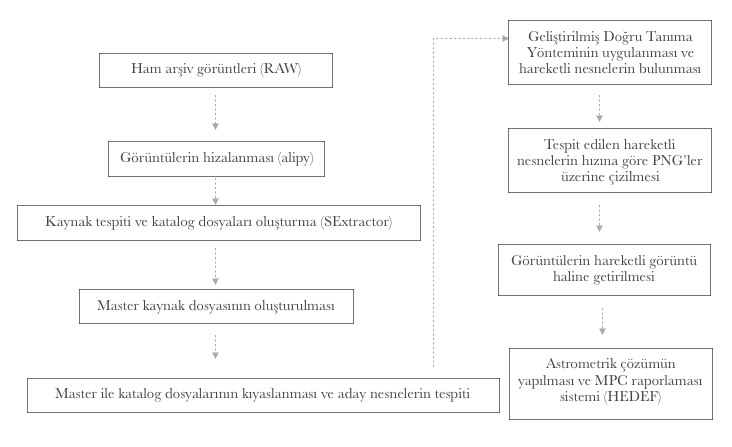
\includegraphics[scale=0.50]{algoritma}
  \caption{Pipeline'nin algoritmasi}
  \label{fig:algoritma}
\end{figure}

\subsection{Goruntulerin Secilmesi}

Pipeline’da kullanilan veri setleri 2500 m. yukseklikteki TUBITAK Ulusal Gozlemevi’nde (TUG) bulunan 100 cm capli T100 teleskobuna bagli Spectral Instruments (SI) 1100 4096 x 4037 px, CCD’sinden elde edilmistir. Yazilimin performansini denetleyebilmek adina veri setlerinin SNR degerlerininin dusuk, orta ve yuksek olmasina ve kalabalik alanli gozlem verilerin secilmesine ozen gosterilmistir. Secilen goruntulerde algoritmamizin isletilmesinde son derece onemli olan gozlem zamani (DATE-OBS), alinan   goruntunun poz suresi (EXPTIME), binning miktari (XBIN, YBIN), boyutu (NAXIS1, NAXIS2) ile ilgili anahtarlarin goruntu basliklarinda olmasi gerekmektedir.

\subsection{Goruntulerin Hizalanmasi} \label{sec:align}

%{\em Hareketli nesnelerin goruntu uzerinde tespiti icin pek cok yontem vardir (ne onlar? bence görüntülerin hizalanması işinin dışına çıkılmamalı). Bunlardan bir kacina ornek vermek gerekirse(!), goruntuler hizalandiktan sonra istifleme islemleri gerceklestirildiginde yildiz, galaksi veya vb. cok uzak nesneler Gunes Sistemi nesnelerine gore  gozlem sureleri baz alindiginda sabit kabul edileceginden, bu istifleme sonrasi asteroid, KY vb. nesneler CCD goruntusu uzerinde cizgi seklinde gorunecektir. Bu cizgilerin tanimlanmasi sonucunda yakin asterodilerin kesfedilmesi mumkundur (Güneş sistemi içerisindeki komet ve asteroid gibi hareketli cisimlerin keşfedilmesi mümkündür). (Benzer şekilde..) Ayrica belirgin bir asterodin takibi ile de diger(?) yildizlar Yer’in ekseni etrafindaki donus yonunun tam tersine dogru (nesneler) yine cizgi halinde gorunecektir. Goruntudeki uzak kaynaklarin herbiri belirli bir yone dogru (dogudan batiya dogru) hareket ederken, asteroidler eger yeterince hareket edebilmislerse cogunlukla farkli yonlere dogru cizgiler olusturacaktir. Ayrica alinan goruntulerin medyanlari alinarak, olusturulan bu medyan goruntunun tum goruntulerden cikarilmasi sonucu da hareketli nesne tespiti yapilabilmektedir \citep{yanagisawa2005}. Fakat bu yontemin verimli calismasi icin maalesef 20’den fazla SNR orani yuksek goruntuye ve cok fazla zamana ihtiyac duyulmaktadir.  Bu yontemlerin cogu icin pipelinelar olusturulabilir ve NEA’lar veya uydularin tespiti icin de zaten boyle calismalar ve yazilimlar bulunmaktadir \citep{vandame2001}. (hareketli cisim tespiti ile görüntü hizalama birleşmiş. bence gereksiz.}


Hizalama adimi ardisik gelen goruntulerdeki hareket eden nesnenin tepiti acisindan onemli bir adimdir. Biz hizalama islemini gerceklestirmek icin, Python programlama dili ile gelistirilmis ve GPL ile dagitilan Malte Tewes’in alipy adli yazilimini kullandik. Alipy’da hizalama islemleri icin, elde ettigi referans katalog dosyasindaki oruntu ile diger goruntulerin katalog dosyasindaki oruntuyu eslestirmek icin \citep{lang2010} calismasini temel alarak scipy afin donusunu veya PyRAF’in geomap/gregister modulunu kullanmaktadir. Bizim icin sadece afin donusumu yeterli olmaktadir. Bu islemin nasil gerceklestiginin basit bir anlatimini Fig.~\ref{fig:hizalama}’te inceleyebilirsiniz. 
\begin{figure}[!t]
  \centering
  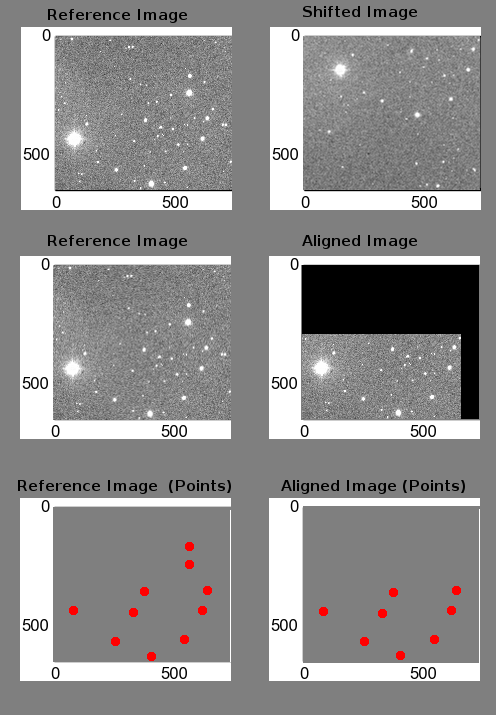
\includegraphics[scale=0.50]{align}
  \caption{Hizalama adimi}
  \label{fig:hizalama}
\end{figure}

\subsection{Hizalanan Goruntulerden Nesne Tespiti}

Gelistirdigimiz pipeline'de hizalama komutu (unless --skip-align) calistirildiktan sonra $X$, $Y$ shift ve $\theta$'ya gore hizalanan goruntuler belirtilen dizin icerisine kayit edilir (atrack/). Artik yuksek hassasiyetle hizalanmis goruntulerden nesne tespti amacimiza uygun hale gelmistir. CCD goruntulerinden kaynak tespiti yapabilen pek cok yazilim vardir. Bunlara ornek verecek olursak; astrometry.net’in image2xy modulu, IRAF’in daofind ve starfind komutlari ve buna benzer pek cok IDL kutuphanesi bulunmaktadir. Fakat, CCD goruntulerden kaynak tespiti yapmak isteyince suphesiz bu konuda hem cok basarili ve de hem de cok hizli olmasi bakimindan ilk akla gelen yazilim SExtractor’dur \citep{bertin1996}. Biz bu calismada SExtractor’un en son surumu olan 2.19.5 surumunu kullandik. Pipeline’da daha sonuk cisimlerin tanimlanmasi, daha fazla hareketli nesnenin tespit edilmesine olanak saglayacaktir. Dolayisiyla fonksiyonlarin yazilmasinda Sextarctror’u kullanirken cesitli tespit parametrelerinin kullaniciya bagli olmasina ozellikle ozen gosterdik. Goruntulerden nesne tespitini N. Cantale’in pysex modulu araciligi ile SExtractor’u kullanarak, daha sonra aday nesnelerin karakteristiklerini incelemek adina, nesnelerin tespit loglarini (FLAGS), nesnelerin goruntu uzerindeki konumlarini (XIMAGE, YIMAGE), akilarini ve hatasini (FLUXAUTO, FLUXERRAUTO), arkaplan degerini (BACKGROUND) ve basiklik degerini (ELONGANTION) herbir nesne icin kendi goruntu dosyasiyla iliskilendirerek katalogladik (SExtractor output).

\subsection{Master Katalog Dosyasi ve Aday Nesnelerin Belirlenmesi} \label{sec:hnak}

Her bir goruntu icin nesne tespiti sonrasi olusan katalog dosyalarindan (*.pysexcat) hareketli nesne adaylarinin belirli bir tolerans degerine gore ayrilmasi gerekmektedir. Bu ayirim sonrasi hareketsiz olan nesnelerden arda kalanlar yalnizca; SEEING’den dolayi merkezi tolerans degerinden fazla oynamis hareketsiz nesneler (cogunlukla yildiz), kozmik isinlardan dolayi asiri yuklenmis bolgeler ve gercek hareketli nesneler olacaktir. Bu islemin gerceklesmesi icin kurguladigimiz algoritma geregi, ilk olarak bir Master Katalog Dosyasin’a (MKD, master.pysexcat) ihtiyac duyulmaktadir. MKD dosyasi aslinda tum goruntulerden olusturulmus katalog dosyalarinin hepsini bir katalog dosyasinda birlestirilmis halidir. Boylelikle her bir goruntudeki her bir nesne MKD icinde belirli bir tolerans degerinden uzak olmamak kosulu ile, kac kez tekrar ediyor kontrol edilir ve eger bu kontrol sonrasinda tolerans icerisinde kalan nesne sayisi 1 adet ise nesnenin hareket ediyor olma olasiligi yuksektir ve Hareketli Nesnelerin Aday Kataloguna  ($HNAK$) kaydedilir (*.cnd). Bu tekrar islemi 1’den fazla ise o bir sabit nesne demektir ve $HNAK$’ya kaydedilmez. Bu islem her bir katalog dosyasinda bulunan her bir nesne icin gerceklestirilir. Islem bittiginde diger bir katalog dosyasina gecilir. Bu islemin matematiksel olarak anlatimi Denklem~\ref{eq:hnak}’de gosterilmistir.

\begin{equation} \label{eq:hnak}
\sum_{n=0}^{n_{\max }}{\sum_{m=0}^{m_{max}}{\sqrt{\left( m_{x}-n_{x} \right)^{2}+\left( m_{y}-n_{y} \right)^{2}}}\leq \; \delta{x}} 
\end{equation}

Denklem~\ref{eq:hnak}’de katalog dosyasi icerisindeki nesneler (n) sirasiyla master dosyasindaki nesnelere (m) uzaklik bakimindan kiyaslaniyorlar. Master dosyasindaki bu kiyaslamanin sonucunda hareketli nesnelerin yalnizca bir kez bu sarti saglamasi gerekir. Tabii bu ornegi aciklamak icin sadece MKD ile kiyaslama esnasinda yalnizca nesnenin toleranstan uzaga kacabilme sarti degerlendirilmemistir. SExtractor'dan nesnelerin karakteristigi ile ilgili farkli degerler de alindigindan bolum~\ref{sec:align}'te bahsetmistik. Eger sadece Denklem~\ref{eq:hnak}'deki uzaklik sartini aday nesne belirlemek icin kullanirsak; pek cok gorus kalitesinden, kozmik isinlardan ve arkaplan dalgalanmalarindan kaynakli nesnelerin de aday nesne kataloguna alinmasina sebep olabiliriz. Bu yuzden istenmeyen bu nesneleri SExtractor'den gelen diger ozelliklerini de dikkate alarak elemek durumundayiz. Bunlardan en onemlileri tabii ki de HNAK'a atilacak nesnelerin saglamasi gereken maksimum FWHM ve minimum FWHM degerleridir. Pipeline'de bu minimum FWHM degeri 1 px olarak belirlenirken,  maksimum FWHM degeri MKD'deki tum nesnelerin FWHM degerinin  medyaninin 2.5 (optional) kati olarak belirlenmistir. Boylelikle SEEING'den bagimsiz olarak hareketli nesneler rahatlikla belirlenebilecektir. Ayrica, her bir nesnenin SNR degeri 2.5 (optional)'dan buyuk olmak durumundadir. Bunlarin yani sira ayrica da SExtractor katalog dosyalarinda bulunan nesnelerin FLAG degerleri, basikligi (ELONGATION) da HNAK'a nesne atilirken degerlendirilmektedir. Tum bu kiyaslamalar GitHub uzerinden paylastigimiz kaynak kodda mevcuttur ($asteroids.py, detect_candidates$).

\subsection{Astronomik Amacli Gelistirilmis Dogru Tanima Yontemi ve Nesne Etiketleme} \label{sec:objecttags}

Literatur incelendiginde farkli dogru tanima algoritmalari bulunmaktadir. Goruntu islemede bunlardan en cok kullanilani Hough donusumu ve bu donusumun varyasyonlaridir (\citep{hough1962}, \citep{ricard1972}). Fakat bizim calismamiza entegre edilebilirdigi acisindan \citep{chen2001}'in calismasiyla ortaya konulmus Dogru Tanima Yontemi (DTY)'nin en uygun yontem oldugunu dusunmekteyiz. Goruntu icerisinde dogru olusturmus noktalarin belirlenebilmesi sebebiyle oncelikle DTY tercih edilmis ve amacimiza uygun olarak gelistirilmistir. DTY, ilgilenilen goruntudeki (ana görüntü değil miydi?) kaynak noktalarina (koordinatlara) uyarlandiginda şu şekilde calisir (Fig.~\ref{fig:hizalama}). Once iki nokta ele alinir, sonra ucuncu bir nokta alinip, bu iki nokta ile dogrudaş olup olmadigi kontrol edilir. Eger alinan uc noktanin dogrudaş oldugu dogrulanirsa bu karşilaştirma ana goruntudeki diger noktalar icin de tekrarlanir. Burada zor olan, uc noktanin dogrudaş olma kriterlerinin belirlenmesidir. Kullanilan yontemde uc noktanin dogrudaş olmasinin birinci koşulu, her bir nokta (vi) ve bu noktaya karşilik gelen koordinatlar vi=(xi , yi) olmak uzere, bu uc noktanin oluşturacagi ucgenin alaninin degerinin sifir veya sifira cok yakin olmasidir. Bu degerleri, uc noktasi bilinen ucgenin alani formulunden hesaplayabiliriz (denklem~\ref{eq:area}).

\begin{figure}[!t]
  \centering
  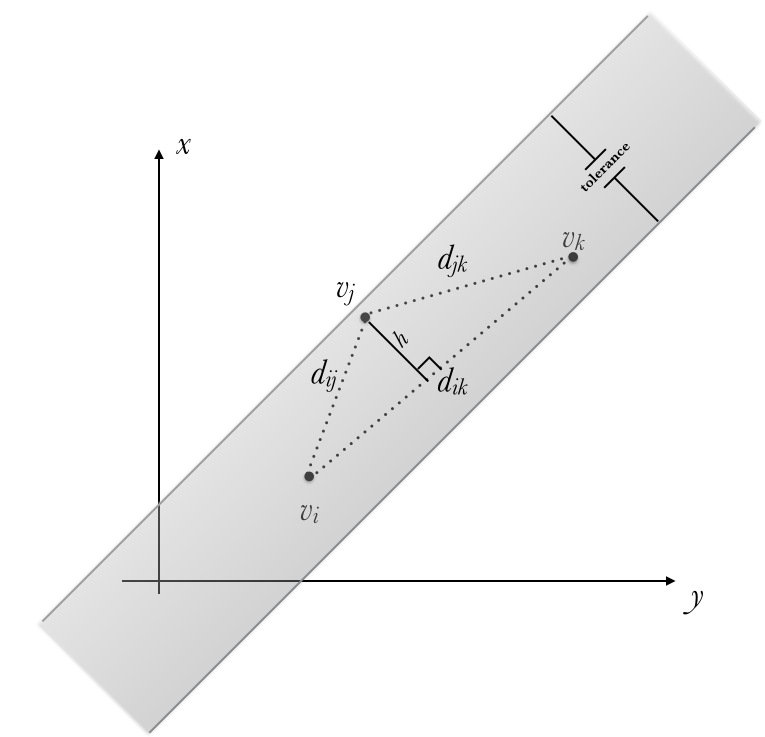
\includegraphics[scale=0.50]{dogru_ucgen}
  \caption{Uc farkli goruntuden secilmis hareketli nesne adaylarinin uzayda sanal dogru uzerinde olusturdugu ucgenin DTY'ye gore semasi}
  \label{fig:dogru_ucgen}
\end{figure}

\begin{equation} \label{eq:area}
\left| z \right|=\frac{1}{2}\left| \left( x_{'}-x_{1} \right)\left( y_{3}-y_{1} \right)-\left( x_{3}-x_{1} \right)\left( y_{2}-y_{1} \right) \right|
\end{equation}

Dijital goruntulerde noktalarin piksellerden  Fig.~\ref{fig:dogru_ucgen} farkli goruntuden secilmis hareketli nesne adaylarinin uzayda sanal dogru uzerinde olusturdugu ucgenin DTY'ye gore semasi olustugu goz onune alindiginda, bu degerin tam olarak sifir olmasa da sifira yakin olmasi beklenir. Ancak bu alanin sifira yakin oldugu her durumda, kullanilan uc noktanin dogrudaş oldugu soylenemez. Uc nokta birbirine cok yakin oldugunda da alan sifira yakin olabilir. Dolayisiyla ikinci bir kritere ihtiyac vardir. Eger secilen uc nokta dogrudas ise bu noktalardan her birinin diger ikisinden gecen dogruya uzakligi (oluşan ucgenin secilen noktasindan karşi kenara inen yuksekligi) da sifira yakin olmalidir. $i$,  $j$, $k$ noktalarindan her biri icin o noktaya karsilik gelen $d_{i->jk}$ yuksekligi bir noktanin bir dogruya olan uzakligi formulu kullanilarak hesaplanir ve en kucuk yukseklik degeri belirlenir (denklem~\ref{eq:height}).

\begin{equation} \label{eq:height}
d_{k_{->}ij}=\frac{\left( x_{j}-x_{i} \right)y_{k}+\left( y_{i}-y_{j} \right)x_{k}+x_{i}y_{j}-x_{j}y_{i}}{\sqrt{\left( x_{j}-x_{i} \right)^{2}+\left( y_{j}-y_{i} \right)^{2}}}
\end{equation}

Eger hesaplanan yukseklik degeri belirli bir tolerans araliginda ise, ucuncu bir kriter olarak, bu uc noktanin birbirlerinden belirli bir eşik degeri kadar uzak olmalari istenir (ucgenin tabani). Bu uc kriterin hepsini saglayan noktalar dogrudaş kabul edilir. Algoritma, ana goruntudeki kaynak noktalarinin (coklu goruntulerden elde edilen potansiyel hareketli cisimlerin koordinatlarinin) dogrudas olup olmadiklarini yukaridaki uc kritere gore degerlendirdikten sonra, bu kaynak noktalarin ayni dogru uzerinde olup olmadigina karar verir \citep{chen2001}. 

\citep{chen2001}'in uyguladigi bu yontem tek bir goruntu uzerindeki surekli noktalari (edges) bulma amaci tasiyordu. Bu yuzden noktalarin arasindaki uzakligin belirlenen limitlerin disinda farkli bir parametre ile denetlenmesinin geregi yoktu. Fakat bizler uzayda hareketli nesneler aradigimiz icin ve bu nesneler belirli bir oz hareket ile CCD uzerinde hareket edeceginden, Fig.~\ref{fig:dogru_ucgen}'te de gosterilmis $d_{ij}$ , $d_{jk}$, $d_{ik}$ dogrularinin vektorel buyukluklerinin birbirleri ile orantili olmasi gerekmektedir. Bu calismada boyle bir kontrol mekanizmasi DTY'den once kullanilmistir. Bu ek kontrol mekanizmasi su sekilde calismaktadir. Dusuk plak eseline sahip CCD goruntusu uzerinde asteroidler mukemmel bir dogru uzerinde yol alirlarlar. Bu yer degistirme de zamana mutlaka bagimlidir. Bu sebeple $\frac{d_{ij}}{∆t_{1}}$ = $\frac{d_{jk}}{∆t_{1}}$ olur. Tabii ki secilen ilk iki nokta ve sonrasinda secilecek ucuncu nokta herhangi ikili nokta cifti olmamalidir. Eger butun noktalarin kombinasyonu olacak sekilde secim yapilirsa ayni dogru uzerinde bulunan ve birbirinden cok uzakta bulunan uclu nokta gruplari da hareketli nesne olarak algilanabilir ve gereksiz bir islem yuku ile karsi karsiya kaliriz. Bunun icin ilk olarak bir baslangic parametresine ihtiyac duyulmaktadir (denklem~\ref{eq:radius}).

\begin{equation} \label{eq:radius}
r\; =\; \left( t_{12}-t_{23} \right)\cdot \frac{V_{\max }}{p.b}
\end{equation}

Denklem~\ref{eq:radius}'te p: piksel olcegini, b: verinin binning degerini temsil etmektedir. Hesaplanacak baslangic parametresi, secilecek olan ilk iki nokta arasindaki uzakligin ne olmasi sorusuyla alakalidir. Burada $V_max$ ‘a herhangi bir deger verilemez. Bu deger arastirilan hareketli nesnelerin turu ve yorungesiyle alakalidir. Bizler bu calismamizda, bu baslangic parametresini Trojan'larin oz hareketleri icin cok hizli sayilabilecek bir deger olan ve ayni zamanda Aten'ler icin de ortalama hizli kabul edilebilir bir oz hareket degeri olan $0.03$ “/s ($V_{max}$)  degerini kullandik. Tabii bu degeri belirlememizde kendi arsivimizden tespit edilen ve yakalayabildigimiz hizli asteroidlerin oz hareketleri de etkili olmustur. Ucuncu nokta icin ise boyle bir kiyaslamaya gerek yoktur. Cunku ucuncu noktanin
Fig.~\ref{fig:hiz} Sabit hizli hareketli nesnenin farkli t zamanindaki konumlari secimi tamamen ilk iki nokta arasindaki hiza baglidir.  Bu durumu daha iyi anlatmasi bakimindan Fig.~\ref{fig:hiz} ve Denklem~\ref{eq:radius} incelenebilir.

\begin{figure}[!t]
  \centering
  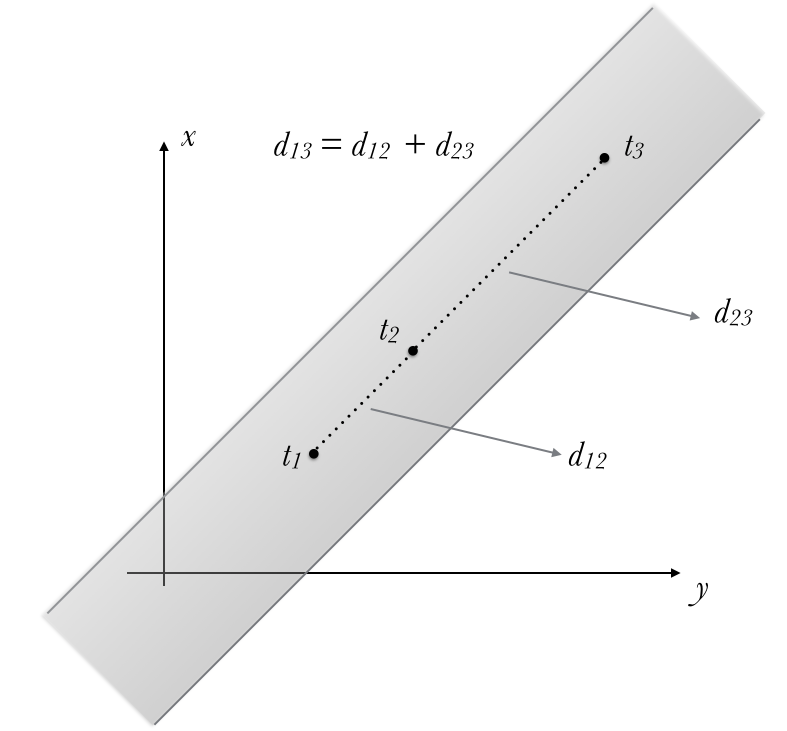
\includegraphics[scale=0.50]{hiz}
  \caption{Sabit hizli hareketli nesnenin farkli t zamanindaki konumlari}
  \label{fig:hiz}
\end{figure}

\begin{equation}
d_{23}=\frac{t_{3}-t_{2}}{t_{2}-t_{1}}\cdot d_{12}
\end{equation}

Denklem~\ref{eq:radius} kurgulamasinin aslinda asteroidlerin gozlem suresi boyunca hizlarinin sabit oldugu varsayimindan ortaya ciktigindan bahsetmistik ($V_{asteroid}$ = $\frac{d_{12}}{∆t_{12}}$ = $\frac{d_{23}}{∆t_{2}}$). CCD goruntulerinin piksellerden (yani kesikli bir iki boyuttan) olustugunun ve de nesnelerin  merkezlerinin ardisik her goruntude -kotu seeing ya da dusuk SNR- den dolayi mukemmel olarak belirlenememesinden kaynaklanan konumdaki hatalar da goz onunde bulundurulursa, ucuncu noktanin konumunun ($d_{23}$ uzunlugu da denebilir) kesin olarak belirlenmesini biraz zora sokmaktadir. Bu yuzden ucuncu noktanin aranmasi gereken konum araligi icin belirli bir tolerans degerinin verilmesi (biz 1 px kullandik) son derece akillica olacaktir. Bu durum yazilimsal olarakta incelemek istenirse $asteroids.py$ modulunde $detect_candidates$ fonksiyonu incelenebilir. 

DTY'nin temel sartlari ile birlikte astronomik hiz ve konum sartlarini da saglayan uclu nesneler bir dizi icerisinde biriktirilir. Bu uclu noktalarin hangilerinin birbirlerinin devami olduguna karar verilir (collectpointsonline foksiyonu), daha sonra birer dogru numarasi verilerek Fig.~\ref{fig:terminal_output}'da oldugu gibi nesnelerin hesaplanan tum ozellikleriyle birlikte kullaniciya cikti verilir.

\begin{figure}[!t]
  \centering
  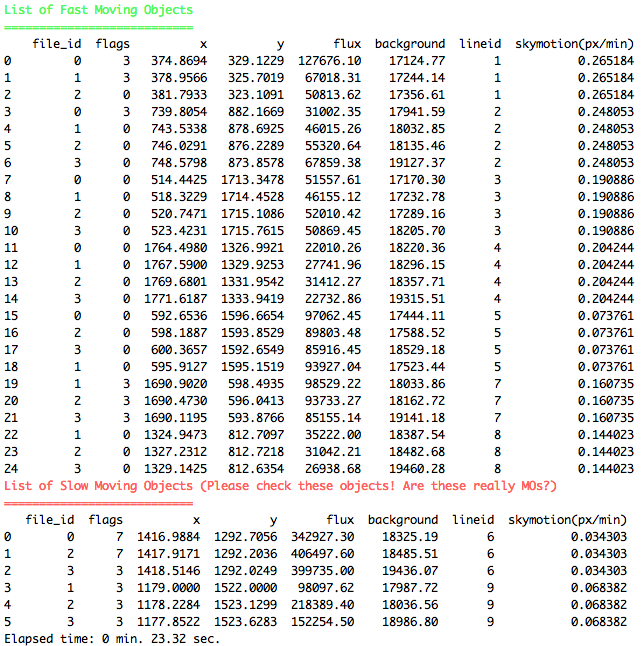
\includegraphics[scale=0.50]{terminal_output}
  \caption{Bir gozlem gecesinden rastgele secilmis 4 goruntuden tespit edilmis hareketli nesneler (Terminal ciktisi)}
  \label{fig:terminal_output}
\end{figure}

\subsection{Belirlenen Hareketli Nesnelerin Gorsellestirilmesi ve Bazi Gorsellestirme Araclari}

Hareketli nesnelerin belirlenmesi ve dogru numaralari ile kullaniciya gosterilmesinden sonra kullanici, tespit edilen bu nesneleri FITS goruntuleri uzerinde gormek isteyebilir ve de hatta animasyon goruntusu olarak hareketli nesneleri izlemek ihtiyaci duyabilir. Cunku Fig.~\ref{fig:terminal_output}'da goruldugu uzere sonuc ciktisinda kirmizi ile isaretlenmis bir takim beklenenin altinda hizlara sahip nesneler bulunmaktadir. Bu nesneler pipeline tarafindan otomatik olarak bizim belirledigimiz minimum hareket hizindan (~0,070 px/min, optional) dusuk nesnelerdir ve bu nesnelerin gercekten hareketli nesne olup olmadigi gorsel olarak teyit edilmelidir.  

Gorsellestime islemi sirasinda FITS (Flexible Image Transport System) goruntuler PNG (Portable Network Graphics) goruntulerine \textit{f2n} adli python modulu ile donusturulmektedir. Bu islem sirasinda tespit edilen nesneler tolerans degerinden buyukse yesil renkte, kucukse kirmizi renkle isaretlenmektedir. Butun goruntulerde bu islemler bittikten sonra istege bagli olarak, donusturulen bu goruntulerden bir animasyon goruntusu imagemagick tarafindan olusturulmaktadir. Fig.~\ref{fig:visual}'de gorsellestirme islemi sonucunda olusturulmus bir PNG goruntusu gosterilmektedir.

\begin{figure}[!t]
  \centering
  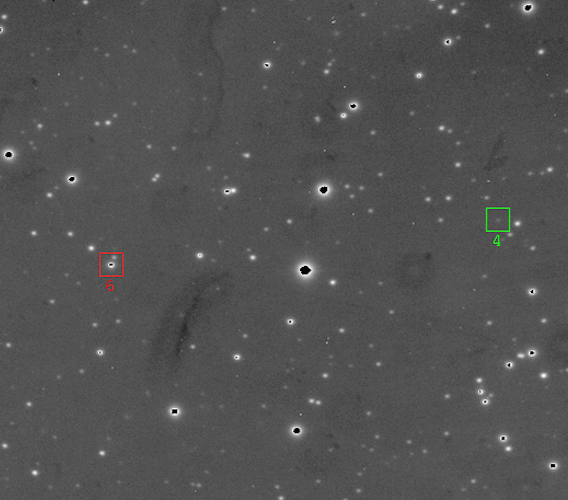
\includegraphics[scale=0.50]{visual}
  \caption{Tespit edilen hareketli nesnelerin hiz kriterine gore farkli renklerde gosterilmesi}
  \label{fig:visual}
\end{figure}

\subsection{Pipeline'da Coklu Islemci (Paralellestirme) Kullanimi}

Gelisen teknolojiyle birlikte, her gecen gun dijitallestirilmis gorsel astronomik veriler ve veri setleri arsiv uzerinde son derece buyuk alanlar kaplamaktadir. Ozellikle gelismis CCD'lerle yapilan gozlemler sonucunda gecelik elde edilen veriler bile Gigabyte'lari hatta Terabyte'lari bulmaktadir. Boylesi buyuk verileri islemek ve analiz etmek icin ciddi islemci hizi ve yuksek hafiza birimlerine ihtiyac duyulmaktadir. Bu donanimlarla birlikte gelistirilen yazilimlarda bu durum goz onunde bulundurularak donanimi etkin ve verimli bir sekilde kullanilmasi adina algoritmanin paralellestirilebilir islemlere zemin saglayacak sekilde gelistirilmesi gerekir. {\em Bu calisma sadece tek bir gecenin gozlem verileri icinden hareketli nesnelerin bulunmasi amaciyla yapilmamistir. Pipeline'in bir arsive uygulanmasi planlanmaktadir.(bu çalışma çalışma/yazılım sadece tek bir gecelik gözlem verileri içinden hareketli nesnelerin bulunmasında kullanılabilecegi gibi arşiv verilerine de uygulanabilecek şekilde tasarlanmıştır öneriydi MK)} Bu sebeple $detect_candidates$ ve $detect_segments$ fonksiyonlarinin tek bir islemciye yuklenilerek calistirilmasi son derece zaman alan bir islem olacaktir. Amacimizin cok sonuk hareketli nesnelerin tespit edilmesi oldugu dusunulurse, SExtractor ile kalabalik bolgelerden tanimlanan nesne sayilari binleri hatta onbinleri bulmaktadir. Bu asamadan sonra $HNAK$'a dusen aday nesneler de yuzleri hatta binleri bulabilmektedir. Ardisik olarak alinmis goruntulerden hareketli nesnenin herhangi bir goruntude tanimlanamama olasiligina karsin da secilen 3 nokta sirasiyla $C(N:Dosya sayisi, 3)$ olmaktadir. Yani N degeri arttikca daha fazla arama islemi gerceklestirilmektedir. Bu sebeple hem zamandan tasarruf etmek, hem de donanimi verimli kullanmak adina pipeline'da $C(N,3)$ kombinasyonlarini tek bir islemci yerine, $C(N,3)/CPUCOUNT$ kadar islemci ile $detect_candidates$ ve $detect_segments$ fonksiyonlari calistirilmaktadir (Fig.~\ref{fig:mp_akis_semasi}).

\begin{figure}[!t]
  \centering
  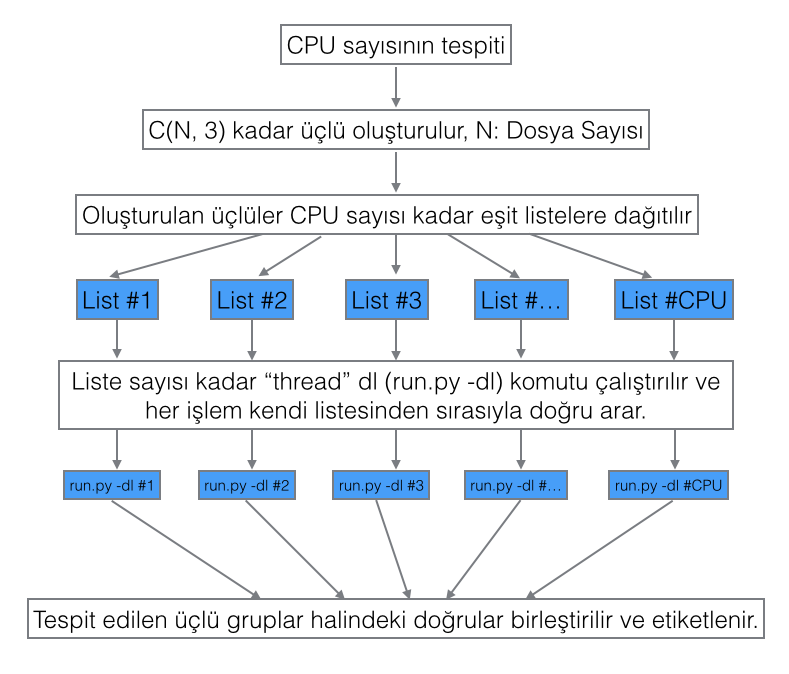
\includegraphics[scale=0.50]{mp_akis_semasi}
  \caption{Paralelize edilmis islemlerin akis semasi}
  \label{fig:mp_akis_semasi}
\end{figure}

\section{Gelecek Hedefler (Future Works)}

Buyuk veri iceren astronomik arsivlerden hareketli nesnelerin, belirlenen algoritmanin gelistirilmesi suretiyle tespiti, bu calisma ile mumkun hale gelmistir. Fakat bu pipeline'i kullanacak kullanici yelpazesi genellikle bilim insanlarindan olusacaktir. Hal boyle bile olsa kullanicilara islemlerin mumkun olan en kisa surede bitirilmesi ve de istenilen komutlarin en kisa surede kolaylikla verilmesi acisindan, bir kullanici dostu grafik arayuz (GUI) sunulmasi da ilerleyen sureclerde dusunulmektedir. GUI'nin yani sira tespit edilen hareketli nesnelerin astrometrik (WCS - World Coordinate System) cozumunun de yapilarak MPC (Minor Planet Center)'ye raporlanmasi adiminin da eklenmesi orta/kısa vadeli hedeflerimiz arasindadir. Bu hedefler sirasiyla asagidaki gibidir.

\begin{itemize}
\item WCS cozumunun tum goruntuler icin yapilmasi
\item Tespit edilen nesnelere XY2RADEC donusumunun uygulanmasi
\item MPC raporlama ozelliginin eklenmesi
\item Kullanici dostu GUI eklenmesi
\end{itemize}

\section{Sonuc ve Tartisma} \label{conclusion}

Gelistirdigimiz yazilim TUG'dan farkli gecelerde alinmis veri setlerine uygulanarak denenmis ve pipeline ile TUG yerleskesinin gorus kalitesi ve $T100$ teleskobunun limit parlakligi ($\approx 21.5^{m}$) da goz onune alinarak, gozlem yapilan bolgeye ait MPC (MPC katalog taraması) taramasi sonucu bulunmasi gereken (beklenen) asteroidler ile karsilastirma yapilarak hareketli nesneler literatur ile dogrulanmistir. Buna ek olarak MPC veritabaninda bulunmayan fakat, yazilimin tespit ettigi hareketli nesneler de tespit edilmistir.

Gelistirilen pipeline; ilgilenilen cisim, bolge ve kullanilan optik araclar da goz onune alindiginda bir takim parametrelerin degistirilmesine ihtiyac duyulabilir. Bu parametreler $atrack.config$ dosyasi icerisinde bulunmaktadir ve 3 ayri baslik altinda kategorilenmistir: $sources$ (nesnelerin sextractor ile tespiti icin gerekli parametreler), $asteroids$ (hareketli nesne olup olmadiginin testi icin gerekli parametreler), $visuals$ (gorsellestirme icin gerekli parametreler). Bu parametlerin degisimine ihtiyac duyulmadigi durumlarda pipeline on tanimli parametrelerle calisacaktir. $sources$ basligi altinda bulunan parametreler bir FITS goruntu uzerindeki nesnelerin dogru bir sekilde tespiti icin gereklidir ve tamamen Sextractor ile alakalidir. Biz bu parametreleri \citep{bertin1996}'in sonuk cisimler icin onerdigi degerlere gore belirledik. Bu sebeple bizim gelistirdigimiz pipeline'da hareketli cisimlerin tespitini etkileyen en onemli parametlerin degisimi ile tespit edilen hareketli nesnelerin sayisini gosterir bir takim tablolar hazirlanmistir gösteren tablolar verilmiştir . Ayrica su kesinlikle unutulmamalidir ki, tespit edilen nesne sayisi sadece bu parametlere bagli degildir. Sextractor parametreleri FITS goruntu uzerindeki tum kaynak noktalari tespiti ettigi durumda maksimum hareketli nesne sayisinin elde edilecegi unutulmamalidir. Elimizdeki $sources$ parametleri bizim kullandigimiz veri seti icin en uygun parametre setidir ve baska veri setleri için degistirilmesi gereke
bilir ve bu
 tamamen ku
llaniciya v
e calisilan veri setine baglidir. Burada irdelenen parametrelerin degisimiyle, hareketli nesnelerin ardisik noktalarinin dogru tanima algoritmasina gore tespit edilip edilemeyecegi ve bu parametrelerle tespit edilen hareketli nesne sayisi arasindaki iliski ortaya konulmustur. Kullanici bu sayede kendi veri setinde hangi deger araliginda parametre degeri belirlemesi konusunda bir fikri olusturacagini dusunmekteyiz. Bu parametrelerin ($TRAVEL_{MIN}$, $HEIGHT_{MAX}$, $\tau$, $SNR$) algoritma icerisinde neleri kontrol ettigi ise Sec.~\ref{sec:detection}'de ayrintili bahsedilmistir. 

$TRAVEL_{MIN}$ ($\delta{x}$) parametresi Sec.~\ref{sec:objecttags}'de ve Eq.~\ref{eq:hnak}'da ayrintili olarak aciklandigi gibi secilen iki noktanin HNAK'a alinma sartini belirtir. Yani hareketli nesne olmanin ilk sartidir. Secilen 3 noktadan herhangi ikisi arasindaki mesafe $\delta{x}$ (px) degerinden az ise o nesne hareketli olarak kabul edilmez ve HNAK'a alinmaz. Tablo~\ref{tab:travelmin}'de 2000CA30 ve Astronomia adli iki veri setine pipeline uygulanarak $\delta{x}$'in degisimiyle tespit edilen hareketli nesne sayisi incelenmistir. Yapilan testlerde arsivimizde hareketli nesne oldugu dogrulanmis en yavas nesnenin iki nokta arasindaki uzakligi 0.3 px olarak belirlenmistir. Fakat farkli veri setlerine bu kadar kucuk bir $\delta{x}$ parametresinin uygulanmasiyla \textit{Slow Detection} sayisinda artma meydana gelecektir. Cunku bu degerin azalmasi hizalamanin mukemmel olamayacagi gercegi ve atmosferik seeingden kaynakli nesnelerin merkez kaymalarindan dolayi HNAK'a cok fazla nesne atilmasina sebep olacak ve olusturulacak dogru icin secilen uc noktalarin kombinasyonlari cok gereğinden fazla artacaktir. Bu durum da yuksek CPU islem gucu ve zamani gerektirdiginden islemi uzatacak ayni zamanda da birbirine cok yakin nesnelerin ayni dogru uzerinde kabul edilmesini saglayacaktir. Yapilan testler ile Tablo ~\ref{tab:travelmin}'de de goruldugu uzere bu deger arttikca \textit{Slow Detection} sayisi artmis ve \textit{True Detection} sayisi azalmistir. Bu calisma sonucunda en optimum yavas hareket eden nesnelerin de tespiti acisindan 0.5 px degeri uygun bir on tanimli parametre olarak secilmistir. Su durum kesinlikle unutumamalidir ki $\delta{x}$ ne kadar kuculurse \textit{Slow Detection} (yavas hareketli nesnelerle birlikte cogunlukla False detectionlar) sayisi artacaktir.

\begin{table}[H]
    \begin{subtable}[h]{0.45\textwidth}
        \centering
        \scalebox{0.5}{
        \begin{tabular}{@{}cccccc@{}}
                 \toprule
                 \multicolumn{6}{c}{\textbf{2000CA30}} \\ \midrule
                 \textbf{$\delta{x}$ (px)} & \textbf{Real} & \textbf{\begin{tabular}[c]{@{}c@{}}Fast True\\ Detection\end{tabular}} & \textbf{\begin{tabular}[c]{@{}c@{}}Fast False \\ Detection\end{tabular}} & \textbf{\begin{tabular}[c]{@{}c@{}}Slow \\ Detection\end{tabular}} & \textbf{\begin{tabular}[c]{@{}c@{}}Elapsed Time\\(HH:MM:SS)\end{tabular}}\\ \midrule
                 0.1 & 4 & 7 & 430 & 449 & 00:20:34 \\
                 0.2 & 4 & 7 & 2 & 45 & 00.02:55 \\
                 0.3 & 4 & 7 & 0 & 8 & 00:01:27  \\
                 0.4 & 4 & 7 & 0 & 4 & 00:01:04 \\
                 \rowcolor{LightCyan}
                 0.5 & 4 & 7 & 0 & 2 & 00:00.59 \\
                 0.6 & 4 & 7 & 0 & 2 & 00:00:57 \\
                 0.7 & 4 & 7 & 0 & 0 & 00:00:51 \\
                 0.8 & 4 & 7 & 0 & 0 & 00:00:51 \\
                 0.9 & 4 & 7 & 0 & 0 & 00:00:53 \\
                 1.00 & 4 & 7 & 0 & 0 & 00:00:52 \\
                 1.10 & 4 & 7 & 0 & 0 & 00:00:51 \\
                 1.20 & 4 & 7 & 0 & 0 & 00:00:53 \\
                 1.30 & 4 & 7 & 0 & 0 & 00:00:53 \\
                 1.40 & 4 & 7 & 0 & 0 & 00:00:51 \\
                 1.50 & 4 & 7 & 0 & 0 & 00:00:50 \\
                 1.60 & 4 & 7 & 0 & 0 & 00:00:53 \\
                 1.70 & 4 & 7 & 0 & 0 & 00:00:51 \\
                 1.80 & 4 & 7 & 0 & 0 & 00:00:53 \\
                 1.90 & 4 & 7 & 0 & 0 & 00:00:53 \\
                 2.00 & 4 & 5 & 0 & 0 & 00:00:53 \\
                 2.10 & 4 & 5 & 0 & 0 & 00:00:53 \\
                 2.20 & 4 & 5 & 0 & 0 & 00:00:57 \\
                 2.30 & 4 & 5 & 0 & 0 & 00:00:51 \\
                 2.40 & 4 & 4 & 0 & 0 & 00:00:52 \\
                 2.50 & 4 & 4 & 0 & 0 & 00:00:51 \\
                 2.60 & 4 & 3 & 0 & 0 & 00:00:52 \\
                 2.70 & 4 & 3 & 0 & 0 & 00:00:52 \\
                 2.80 & 4 & 2 & 0 & 0 & 00:00:50 \\
                 2.90 & 4 & 2 & 0 & 0 & 00:00:51 \\
                 3.00 & 4 & 2 & 0 & 0 & 00:00:51 \\
        \end{tabular}
        }
        \caption{2000CA30}
        \label{tab:2000CA30_travelmin}
    \end{subtable}
    \hfill
    \begin{subtable}[h]{0.45\textwidth}
        \centering
        \scalebox{0.5}{
        \begin{tabular}{@{}cccccc@{}}
                 \toprule
                 \multicolumn{6}{c}{\textbf{Astronomia}} \\ \midrule
                 \textbf{$\delta{x}$ (px)} & \textbf{Real} & \textbf{\begin{tabular}[c]{@{}c@{}}Fast True\\ Detection\end{tabular}} & \textbf{\begin{tabular}[c]{@{}c@{}}Fast False \\ Detection\end{tabular}} & \textbf{\begin{tabular}[c]{@{}c@{}}Slow \\ Detection\end{tabular}} & \textbf{\begin{tabular}[c]{@{}c@{}}Elapsed Time\\(HH:MM:SS)\end{tabular}}\\ \midrule
                0.1 & 3 & 3 & 3 & 38 & 00:00:02 \\
                0.2 & 3 & 3 & 2 & 4 & 00:00:24 \\
                0.3 & 3 & 2 & 0 & 0 & 00:00:23 \\
                0.4 & 3 & 2 & 0 & 0 & 00:00:23 \\
                \rowcolor{LightCyan}
                0.5 & 3 & 2 & 0 & 0 & 00:00:23 \\
                0.6 & 3 & 2 & 0 & 0 & 00:00:23 \\
                0.7 & 3 & 2 & 0 & 0 & 00:00:23 \\
                0.8 & 3 & 2 & 0 & 0 & 00:00:23 \\
                0.9 & 3 & 2 & 0 & 0 & 00:00:23 \\
                1.00 & 3 & 2 & 0 & 0 & 00:00:23 \\
                1.10 & 3 & 2 & 0 & 0 & 00:00:23 \\
                1.20 & 3 & 2 & 0 & 0 & 00:00:23 \\
                1.30 & 3 & 1 & 0 & 0 & 00:00:23 \\
                1.40 & 3 & 1 & 0 & 0 & 00:00:23 \\
                1.50 & 3 & 1 & 0 & 0 & 00:00:24 \\
                1.60 & 3 & 1 & 0 & 0 & 00:00:24 \\
                1.70 & 3 & 0 & 0 & 0 & 00:00:11 \\
                1.80 & 3 & 0 & 0 & 0 & 00:00:11 \\
                1.90 & 3 & 0 & 0 & 0 & 00:00:11 \\
                2.00 & 3 & 0 & 0 & 0 & 00:00:11 \\
                2.10 & 3 & 0 & 0 & 0 & 00:00:11 \\
                2.20 & 3 & 0 & 0 & 0 & 00:00:11 \\
                2.30 & 3 & 0 & 0 & 0 & 00:00:11 \\
                2.40 & 3 & 0 & 0 & 0 & 00:00:11 \\
                2.50 & 3 & 0 & 0 & 0 & 00:00:11 \\
                2.60 & 3 & 0 & 0 & 0 & 00:00:11 \\
                2.70 & 3 & 0 & 0 & 0 & 00:00:11 \\
                2.80 & 3 & 0 & 0 & 0 & 00:00:11 \\
                2.90 & 3 & 0 & 0 & 0 & 00:00:11 \\
                3.00 & 3 & 0 & 0 & 0 & 00:00:11 \\
        \end{tabular}
        }
        \caption{Astronomia}
        \label{tab:astronomia_travelmin}
    \end{subtable}
    \caption{$\delta{x}$ ($TRAVEL_{min}$) parametresinin farkli veri setlerinde degisimi ve kiyaslanmasi}
    \label{tab:travelmin}
\end{table}

Tablo ~\ref{tab:heightmax}'de Fig.~\ref{fig:dogru_ucgen}'de aciklanan $h$ ($HEIGHT_{MAX}$) parametresinin piksel cinsinden degisimine gore tespit edilen cisim miktari iki farklı veri seti ile karsilastirilmistir (2000CA30, Astronomia). Bu karsilastirma sonucunda bizim belirledigimiz on tanimli parametre dogrulugu MPC veri tabani ve goz ile teyit edilmis hareketli nesnenin tespit edildigi 0.10 px degeri secilmistir. Burada dikkat edilmesi gereken ve elde edilen sonuclar sunu gostermektedir, teoride de beklendigi gibi, $h_max$ degerinin artmasiyla bulunabilecek hareketli nesne sayisinin azaldigidir. Cunku $h_max$ parametresinin artmasi ardisik gelen 3 noktanin ayni dogru uzerinde bulunma olasiligini azalmaktadir.

\begin{table}[H]
    \begin{subtable}[h]{0.45\textwidth}
        \centering
        \scalebox{0.5}{
        \begin{tabular}{@{}cccccc@{}}
                 \toprule
                 \multicolumn{6}{c}{\textbf{2000CA30}} \\ \midrule
                 \textbf{$h_{max}$ (px)} & \textbf{Real} & \textbf{\begin{tabular}[c]{@{}c@{}}Fast True\\ Detection\end{tabular}} & \textbf{\begin{tabular}[c]{@{}c@{}}Fast False \\ Detection\end{tabular}} & \textbf{\begin{tabular}[c]{@{}c@{}}Slow \\ Detection\end{tabular}} & \textbf{\begin{tabular}[c]{@{}c@{}}Elapsed Time\\(HH:MM:SS)\end{tabular}}\\ \midrule
                        0.05 & 4 & 6 & 0 & 4 & 00:01:11 \\
                        \rowcolor{LightCyan}
                        0.10 & 4 & 7 & 0 & 6 & 00:01:09 \\
                        0.15 & 4 & 7 & 1 & 11 & 00:01:08 \\
                        0.20 & 4 & 7 & 1 & 12 & 00:01:12 \\
                        0.25 & 4 & 7 & 2 & 16 & 00:01:12 \\
                        0.30 & 4 & 7 & 2 & 17 & 00.01:23 \\
                        0.35 & 4 & 7 & 2 & 19 & 00:01.20 \\
                        0.40 & 4 & 7 & 3 & 21 & 00:01:24 \\
                        0.45 & 4 & 7 & 4 & 27 & 00:01:23 \\
                        0.50 & 4 & 7 & 4 & 28 & 00:01:23 \\
                        0.55 & 4 & 7 & 4 & 28 & 00:01:08 \\
                        0.60 & 4 & 7 & 4 & 28 & 00.01:10 \\
                        0.65 & 4 & 7 & 4 & 29 & 00:01:07 \\
                        0.70 & 4 & 7 & 6 & 27 & 00:01:09 \\
                        0.75 & 4 & 7 & 6 & 28 & 00:01:09 \\
                        0.80 & 4 & 7 & 6 & 28 & 00:01:13 \\
                        0.85 & 4 & 7 & 7 & 29 & 00:01:13 \\
                        0.90 & 4 & 7 & 8 & 28 & 00:01:10 \\
                        0.95 & 4 & 7 & 9 & 29 & 00:01:08 \\
                        1.00 & 4 & 7 & 9 & 29 & 00:01:08 \\
        \end{tabular}
        }
        \caption{2000CA30}
        \label{tab:2000CA30_hmax}
    \end{subtable}
    \hfill
    \begin{subtable}[h]{0.45\textwidth}
        \centering
        \scalebox{0.5}{
        \begin{tabular}{@{}cccccc@{}}
                 \toprule
                 \multicolumn{6}{c}{\textbf{Astronomia}} \\ \midrule
                 \textbf{$h_{max}$ (px)} & \textbf{Real} & \textbf{\begin{tabular}[c]{@{}c@{}}Fast True\\ Detection\end{tabular}} & \textbf{\begin{tabular}[c]{@{}c@{}}Fast False \\ Detection\end{tabular}} & \textbf{\begin{tabular}[c]{@{}c@{}}Slow \\ Detection\end{tabular}} & \textbf{\begin{tabular}[c]{@{}c@{}}Elapsed Time\\(HH:MM:SS)\end{tabular}}\\ \midrule
                        0.05 & 3 & 2 & 0 & 0 & 00:00:23 \\
                        \rowcolor{LightCyan}
                        0.10 & 3 & 2 & 0 & 0 & 00:00:23 \\
                        0.15 & 3 & 2 & 0 & 0 & 00:00:23 \\
                        0.20 & 3 & 2 & 0 & 0 & 00:00:23 \\
                        0.25 & 3 & 2 & 0 & 0 & 00:00:23 \\
                        0.30 & 3 & 2 & 0 & 2 & 00:00:23 \\
                        0.35 & 3 & 2 & 0 & 2 & 00:00:23 \\
                        0.40 & 3 & 2 & 0 & 2 & 00:00:23 \\
                        0.45 & 3 & 2 & 0 & 3 & 00:00:23 \\
                        0.50 & 3 & 2 & 0 & 3 & 00:00:23 \\
                        0.55 & 3 & 2 & 0 & 3 & 00:00:23 \\
                        0.60 & 3 & 3 & 0 & 3 & 00:00:23 \\
                        0.65 & 3 & 3 & 0 & 3 & 00:00:23 \\
                        0.70 & 3 & 3 & 0 & 3 & 00:00:24 \\
                        0.75 & 3 & 3 & 0 & 3 & 00:00:23 \\
                        0.80 & 3 & 3 & 0 & 3 & 00:00:23 \\
                        0.85 & 3 & 3 & 5 & 18 & 00:00:47 \\
                        0.90 & 3 & 3 & 0 & 3 & 00:00:22 \\
                        0.95 & 3 & 3 & 0 & 3 & 00:00:24 \\
                        1.00 & 3 & 3 & 0 & 3 & 00:00:23 \\
        \end{tabular}
        }
        \caption{Astronomia}
        \label{tab:astronomia_hmax}
    \end{subtable}
    \caption{$HEIGHTMAX$ ($h_{max}$) parametresinin farkli veri setlerinde degisimi ve kiyaslanmasi}
    \label{tab:heightmax}
\end{table}

Secilen ucuncu noktanin hesaplanan degerden ne kadar bir sapma ile gercek konumunda olacagini denetleyen $\tau$ degeri Sec. ~\ref{sec:hnak}'da ile ayrintili olarak aciklanmisti. Tablo ~\ref{tab:tau}'da pipelinenin ilgili veri setlerine uygulanmasi sonucunda en optimum sure ve hareketli sayisinin bulunmasi bakimindan $1.00 px$ degerin on tanimli deger olmasi kararlanmistir (mavi satirlar secilen on tanimli degerleri gostermektedir). Bu sonuclar ise $\tau$ degerinin artmasiyla ucuncu noktanin daha genis bir cap araliginda taranacagi belirtilmektedir ve bu sebeple Tablo ~\ref{tab:tau}'da goruldugu gibi \textit{Slow Detection} miktarini artırmaktadir. Bu da tespit edilen nesnelerin hareketli nesne olup olmadigi konusunda net bir sey soylenmesini zorlastirmaktadir. Bu degerin kucuk tutulmasi ucuncu noktanin hesaplanan bolgede olacagini belirteceginden islem hem cok hizli hem de guvenilir sonuclar verecektir. Daha ayrntili bilgi icin Sec. ~\ref{sec:objecttags} ve Fig.~\ref{fig:hiz} incelenebilir.

\begin{table}[H]
    \begin{subtable}[h]{0.45\textwidth}
        \centering
        \scalebox{0.5}{
        \begin{tabular}{@{}cccccc@{}}
                 \toprule
                 \multicolumn{6}{c}{\textbf{2000CA30}} \\ \midrule
                 \textbf{$\tau$ (px)} & \textbf{Real} & \textbf{\begin{tabular}[c]{@{}c@{}}Fast True\\ Detection\end{tabular}} & \textbf{\begin{tabular}[c]{@{}c@{}}Fast False \\ Detection\end{tabular}} & \textbf{\begin{tabular}[c]{@{}c@{}}Slow \\ Detection\end{tabular}} & \textbf{\begin{tabular}[c]{@{}c@{}}Elapsed Time\\(HH:MM:SS)\end{tabular}}\\ \midrule
                 0.25 & 4 & 7 & 0 & 2 & 00:01:25 \\
                 0.50 & 4 & 7 & 0 & 4 & 00:01:22 \\
                 0.75 & 4 & 7 & 0 & 6 & 00:01:23 \\
                 \rowcolor{LightCyan}
                 1.00 & 4 & 7 & 0 & 6 & 00:01:23 \\
                 1.25 & 4 & 7 & 1 & 8 & 00:01:23 \\
                 1.50 & 4 & 7 & 1 & 9 & 00:01:21 \\
                 1.75 & 4 & 7 & 1 & 11 & 00:01:21 \\
                 2.00 & 4 & 7 & 2 & 11 & 00:01:20 \\
                 2.25 & 4 & 7 & 2 & 13 & 00:01:18 \\
                 2.50 & 4 & 7 & 2 & 13 & 00:01:20 \\
                 2.75 & 4 & 7 & 2 & 15 & 00:01:10 \\
                 3.00 & 4 & 7 & 2 & 14 & 00:01:13 \\
                 3.25 & 4 & 7 & 3 & 14 & 00:01:13 \\
                 3.50 & 4 & 7 & 4 & 12 & 00:01:10 \\
                 3.75 & 4 & 7 & 4 & 13 & 00:01:21 \\
                4.00 & 4 & 7 & 4 & 14 & 00:01:21
        \end{tabular}
        }
        \caption{2000CA30}
        \label{tab:2000CA30_tau}
    \end{subtable}
    \hfill
    \begin{subtable}[h]{0.45\textwidth}
        \centering
        \scalebox{0.5}{
        \begin{tabular}{@{}cccccc@{}}
                 \toprule
                 \multicolumn{6}{c}{\textbf{Astronomia}} \\ \midrule
                 \textbf{$\tau$ (px)} & \textbf{Real} & \textbf{\begin{tabular}[c]{@{}c@{}}Fast True\\ Detection\end{tabular}} & \textbf{\begin{tabular}[c]{@{}c@{}}Fast False \\ Detection\end{tabular}} & \textbf{\begin{tabular}[c]{@{}c@{}}Slow \\ Detection\end{tabular}} & \textbf{\begin{tabular}[c]{@{}c@{}}Elapsed Time\\(HH:MM:SS)\end{tabular}}\\ \midrule
                 0.25 & 4 & 7 & 0 & 2 & 00:01:25 \\
                 0.50 & 4 & 7 & 0 & 4 & 00:01:22 \\
                 0.75 & 4 & 7 & 0 & 6 & 00:01:23 \\
                 \rowcolor{LightCyan}
                 1.00 & 4 & 7 & 0 & 6 & 00:01:23 \\
                 1.25 & 4 & 7 & 1 & 8 & 00:01:23 \\
                 1.50 & 4 & 7 & 1 & 9 & 00:01:21 \\
                 1.75 & 4 & 7 & 1 & 11 & 00:01:21 \\
                 2.00 & 4 & 7 & 2 & 11 & 00:01:20 \\
                 2.25 & 4 & 7 & 2 & 13 & 00:01:18 \\
                 2.50 & 4 & 7 & 2 & 13 & 00:01:20 \\
                 2.75 & 4 & 7 & 2 & 15 & 00:01:10 \\
                 3.00 & 4 & 7 & 2 & 14 & 00:01:13 \\
                 3.25 & 4 & 7 & 3 & 14 & 00:01:13 \\
                 3.50 & 4 & 7 & 4 & 12 & 00:01:10 \\
                 3.75 & 4 & 7 & 4 & 13 & 00:01:21 \\
                4.00 & 4 & 7 & 4 & 14 & 00:01:21 \\
        \end{tabular}
        }
        \caption{Astronomia}
        \label{tab:astronomia_tau}
    \end{subtable}
    \caption{$\tau$ parametresinin farkli veri setlerinde degisimi ve kiyaslanmasi}
    \label{tab:tau}
\end{table}

Haraketli nesnelerin tespiti esnasinda, Sextractor'un cok sonuk cisim olarak tespit etmis oldugu fakat gercekte kotu gorus kalitesi ve arkaplan dalgalanmalari sebebiyle $HNAK$'a dusmus pek cok nesne olmaktadir. İlgilenilen nesnelerin gercekten "nesne" olup olmadiginin tespiti acisindan $SNR$ (Signal-to-noise ratio, S/R) degeri son derece onemlidir. Bu sebeple $SNR$ parametresi belirlenen degerden kucuk ise o nesne $HNAK$'a alinmaz ve bu sayede algoritmanin uygulanacagi ilgili uclu nokta kombinasyonlari azalır, uzun bir CPU isleminden kacinilarak zaman tasarrufu saglanır. İlgli verilere pipeline cesitli $SNR$ degerlerinde uygulanarak, tespit edilen hareketli nesneler Tablo ~\ref{tab:snr}'de verilmistir. Yapilan incelemeler sonucunda $SNR$ on tanimli degerinin, hem sonuk cisimlerin kacirilmamasi hem de CPU islem yogunlu bakimindan en optimum parametre olmasi sebebiyle $10$ degerinin olmasi tercih edilmiştir. Tablo ~\ref{tab:snr}'de de goruldugu uzere $SNR$ degerinin artmasiyla tespit edilen hareketli nesne miktari azalmaktadir. İlgilenen cismin parlak olmasi durumunda bu degerin artirilmasini tavsiye etmekteyiz. Aksi halde bu calisma ile belirlenen on tanimli deger sonuk cisim taramalari icin optimum deger olacaktir. Daha sonuk cisimler aranacaksa islem zamaninin artacagi goz onunde bulundurularak, bu deger dusurulebilir.

\begin{table}[H]
    \begin{subtable}[h]{0.45\textwidth}
        \centering
        \scalebox{0.5}{
        \begin{tabular}{@{}cccccc@{}}
                 \toprule
                 \multicolumn{6}{c}{\textbf{2000CA30}} \\ \midrule
                 \textbf{$SNR$} & \textbf{Real} & \textbf{\begin{tabular}[c]{@{}c@{}}Fast True\\ Detection\end{tabular}} & \textbf{\begin{tabular}[c]{@{}c@{}}Fast False \\ Detection\end{tabular}} & \textbf{\begin{tabular}[c]{@{}c@{}}Slow \\ Detection\end{tabular}} & \textbf{\begin{tabular}[c]{@{}c@{}}Elapsed Time\\(HH:MM:SS)\end{tabular}}\\ \midrule
                 2.5 & 4 & 7 & 0 & 6 & 00:01:23 \\
                 5 & 4 & 7 & 0 & 6 & 00:01:09 \\
                 7.5 & 4 & 7 & 0 & 6 & 00:01:23 \\
                 \rowcolor{LightCyan}
                 10 & 4 & 7 & 0 & 6 & 00:01:08 \\
                 12.5 & 4 & 6 & 0 & 6 & 00:01:22 \\
                 15 & 4 & 5 & 0 & 6 & 00:01:04 \\
                 17.5 & 4 & 5 & 0 & 6 & 00:01:09 \\
                 20 & 4 & 4 & 0 & 6 & 00:00:56 \\
                 22.5 & 4 & 3 & 0 & 6 & 00:00:49 \\
                 25 & 4 & 3 & 0 & 5 & 00:00:49 \\
                 27.5 & 4 & 3 & 0 & 5 & 00:00:46 \\
                 30 & 4 & 2 & 0 & 6 & 00:00:46 \\
                 32.5 & 4 & 2 & 0 & 6 & 00:00:42 \\
                 35 & 4 & 2 & 0 & 6 & 00:00:43 \\
                 37.5 & 4 & 2 & 0 & 5 & 00:00:40 \\
                 40 & 4 & 2 & 0 & 5 & 00:00:42 \\

        \end{tabular}
        }
        \caption{2000CA30}
        \label{tab:2000CA30_snr}
    \end{subtable}
    \hfill
    \begin{subtable}[h]{0.45\textwidth}
        \centering
        \scalebox{0.5}{
        \begin{tabular}{@{}cccccc@{}}
                 \toprule
                 \multicolumn{6}{c}{\textbf{Astronomia}} \\ \midrule
                 \textbf{$SNR$} & \textbf{Real} & \textbf{\begin{tabular}[c]{@{}c@{}}Fast True\\ Detection\end{tabular}} & \textbf{\begin{tabular}[c]{@{}c@{}}Fast False \\ Detection\end{tabular}} & \textbf{\begin{tabular}[c]{@{}c@{}}Slow \\ Detection\end{tabular}} & \textbf{\begin{tabular}[c]{@{}c@{}}Elapsed Time\\(HH:MM:SS)\end{tabular}}\\ \midrule
                 2.5 & 3 & 2 & 0 & 0 & 00:00:23 \\
                 5 & 3 & 2 & 0 & 0 & 00:00:23 \\
                 7.5 & 3 & 2 & 0 & 0 & 00:00:23 \\
                 \rowcolor{LightCyan}
                 10 & 3 & 2 & 0 & 0 & 00:00:23 \\
                 12.5 & 3 & 2 & 0 & 0 & 00:00:23 \\
                 15 & 3 & 2 & 0 & 0 & 00:00:23 \\
                 17.5 & 3 & 2 & 0 & 0 & 00:00:22 \\
                 20 & 3 & 2 & 0 & 0 & 00:00:22 \\
                 22.5 & 3 & 2 & 0 & 0 & 00:00:23 \\
                 25 & 3 & 2 & 0 & 0 & 00:00:23 \\
                 27.5 & 3 & 2 & 0 & 0 & 00:00:23 \\
                 30 & 3 & 2 & 0 & 0 & 00:00:29 \\
                 32.5 & 3 & 2 & 0 & 0 & 00:00:26 \\
                 35 & 3 & 2 & 0 & 0 & 00:00:27 \\
                 37.5 & 3 & 2 & 0 & 0 & 00:00:26 \\
                 40 & 3 & 2 & 0 & 0 & 00:00:26 \\
        \end{tabular}
        }
        \caption{Astronomia}
        \label{tab:astronomia_snr}
    \end{subtable}
    \caption{$SNR$ parametresinin farkli veri setlerinde degisimi ve kiyaslanmasi}
    \label{tab:snr}
\end{table}

Tum bu sonuclar gosteriyor ki, her veri seti ve her ilgilenilen cisim farkli on tanimli parametrelere ihtiyac duymaktadir. Burada belirlenen parametreler veri setleri uzerinde iyi calisilmis hareketli nesnelerin bulunmasi icin idealdir tabii Sextractor parametrelerinin de degistirilmesi gerektigi unutulmamalidir. Bu pipeline ile hareketli nesneler hizli bir sekilde belirlenebilir ve astrometrisi ve hatta fotometrisi dahi hizli bir sekilde yapilabilir. Bu da piyasada bulunan kapali kaynak kodlu yazilimlarin yani sira kullanicilarin hizli, ucretsiz ve de geri bildirimler sayesinde gittikce guvenilir olarak gelisen bir yazilimi kullanmasini saglayacagi icin son derece onemlidir. A-Track elbette bu an beta asamasindadir fakat bu alanla ilgilenen gokbilimcilerin kullanmasiyla kararli hale donusecegi kanisindayiz.

\section*{Acknowledgements} \label{thanks}
Bu proje 114F477 numarasi ile TUBITAK tarafindan destektenmektedir. Bu projeye verdikleri destekten dolayi basta TÜBİTAK'a, Akdeniz Üniversitesi Fen Fakültesi Uzay Bilimleri ve Teknolojileri Bolumu'ne ve ayrica projeye destek veren tum bilim adamlari ve beta test kullanicilarina tesekkur ederiz. Also, we thank to TUBITAK for a partial support in using T100 telescope with project number <TUG proje no>. 

Gibi birsey kullanmamiz lazim. Tabii bu projede kullanilip kapatilmaya ihtiyac duyuluyorsa.

\section*{References}

\bibliography{a-track.bib}

\end{document}






